\documentclass[8.01x]{subfiles}
\begin{document}

\chapter{Week 2: Homework 2}

\section{Problem 1: Roundtrip by plane}

An airplane makes a roundtrip between point A and point B (starting at A). The purpose of this problem is to figure out if the roundtrip will take longer without wind or with wind. Let the distance between A and B be $d$ and the speed of the plane relative to air be $v$.

``(a) First, assume there is no wind. How long does it take to finish a round trip between A and B (starting at A)? Express your answer as a function of d and v as needed.''

The distance is $d$, the velocity $v$, and since there is no wind, both parts of the trip take equal time, so we simply double the time taken for the one-way trip:

\begin{equation}
t = 2 \frac{d}{v}
\end{equation}

``(b) Now, assume that the wind is blowing in the direction from A to B. How long does it take to finish a round trip between A and B (starting at A), with the wind? Let the distance between A and B be $d$, the speed of the plane relative to air be $v$, and the speed of the wind be $w$ (where $w < v$). Express your answer as a function of d, v, or w as needed.''

The wind blows with the velocity for one part of the trip (net velocity is $v + w$), and against the other (net velocity $v - w$). We add up the two, and that's really it:

\begin{equation}
t = \frac{d}{v + w} + \frac{d}{v - w}
\end{equation}

``Reflect on your answers: What would happen if the wind speed became so high that $w = v$? How would your answer change if the wind were blowing in the direction from B to A?''

In the first case, a plane flying against the wind would stand still, relative to the Earth.\\
If the direction of the wind were reversed from above, the round-trip time should be the same: we would simply change the order of the two fractions, but addition is commutative, so the sum is the same.

\section{Problem 2: Passing planes in flight}

``The velocities of airplanes A and B are measured with respect to a frame of reference S fixed to the ground as shown. Airplane A is traveling northeast ($\ang{45}$ measured counterclockwise from the $x$ axis) with a speed of $v_A = \SI{140}{m/s}$ and airplane B is traveling southeast ($\ang{45}$ measured clockwise from the $x$ axis) with a speed of $v_B = \SI{240}{m/s}$.

\begin{center}
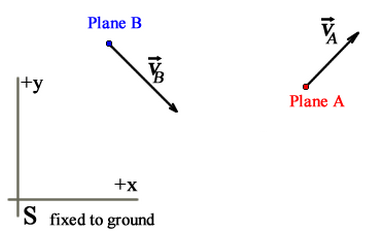
\includegraphics[scale=0.7]{Graphics/h2p2_1}
\end{center}

``(a) What are the components of the velocity of each airplane $\vec{v_A}$ and $\vec{v_B}$ in the xy-coordinate system of the stationary frame S?''

Because the system is fixed as shown, this is simply a vector decomposition problem.

\begin{align}
v_{Ax} &= v_A \cos(\ang{45})\\
v_{Ay} &= v_A \sin(\ang{45})\\
v_{Bx} &= v_B \cos(-\ang{45})\\
v_{By} &= v_B \sin(-\ang{45})
\end{align}

``(b) Consider the frame of reference S' fixed to airplane B. Find $\vec{v_{AB}}$, the velocity of aircraft A as seen from an observer flying in aircraft B?''

\begin{center}
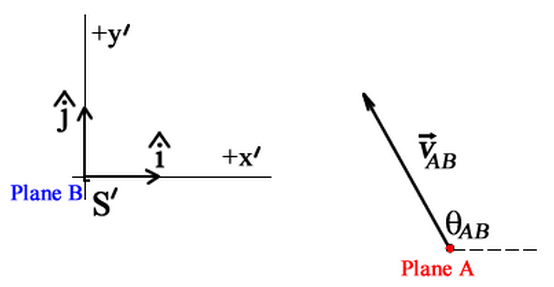
\includegraphics[scale=0.6]{Graphics/h2p2_2}
\end{center}

Let's see. First, a warning: I want to point out that my method here might be overkill... and very ugly. The reason is that this is the first exercise I do these transformations in, and I want to learn how to do them in general, not just in this one case, so I went the full, ugly way.

I will first calculate the transformation from S to S', so that we understand the reference frame we work in. Because the plane is moving relative to S in two dimensions, we need to use a Galilean transformation on both axes separately, using vector decomposition.

The transformation for a single axis $x$ in one-dimensional motion is $x' = x - v t$, so we apply that concept to both axes using the decomposed velocity vector $v_B$, which represents the velocity relative to the ground (reference frame S):

\begin{align}
x' &= x - v_{Bx} t = x - v_B \cos(-\ang{45}) t\\
y' &= y - v_{By} t = y - v_B \sin(-\ang{45}) t\\
\end{align}
	
Let's now attempt to define $v_A$ in terms of $x'$ and $y'$, in other words, $v_{AB}$ as notated in the problem ($v_A$ as seen by plane B).\\
In terms of the components in reference frame S, $v_A$ is

\begin{equation}
v_A = v_{Ax} \hat{x} + v_{Ay} \hat{y} = \frac{d(A_x)}{dt} \hat{x} + \frac{d(A_y)}{dt} \hat{y}
\end{equation}

We know the velocities, we know that the acceleration is 0, and so we can find the position equations simply by multiplying the velocity by $t$, assuming $x_0 = 0$ and $y_0 = 0$. (That should be irrelevant is this context, since we are taking the derivative of them, so that constants disappear.)

\begin{equation}
v_A = \frac{d(v_A \cos(\ang{45}) t)}{dt} \hat{x} + \frac{d(v_A \sin(\ang{45}) t)}{dt} \hat{y}
\end{equation}

We then apply the transformation to S' by subtracting $v_{Bx} t$ and $v_{By} t$ respectively, and then calculate the derivative and simplify:

\begin{align}
v_{AB} = \frac{d(v_A \cos(\ang{45}) t - v_B \cos(-\ang{45}) t)}{dt} \hat{x} + \frac{d(v_A \sin(\ang{45}) t - v_B \sin(-\ang{45}) t)}{dt} \hat{y}\\
v_{AB} = (v_A \cos(\ang{45}) - v_B \cos(-\ang{45})) \hat{x} + (v_A \sin(\ang{45}) - v_B \sin(-\ang{45})) \hat{y}\\
v_{AB} = (v_{Ax} - v_{Bx}) \hat{x} + (v_{Ay} - v_{By}) \hat{y}
\end{align}

Well, that's one long derivation for something we could have guessed! We need some numerical values for the components, or the answer becomes way too ugly (too many terms and too many parenthesis to keep track of).

\begin{align}
v_{Ax} &= 140 \cos(\ang{45}) \approx \SI{98.995}{m/s}\\
v_{Ay} &= 140 \sin(\ang{45}) \approx \SI{98.995}{m/s}\\
v_{Bx} &= 240 \cos(-\ang{45}) \approx \SI{169.706}{m/s}\\
v_{By} &= 240 \sin(-\ang{45}) \approx \SI{-169.706}{m/s}
\end{align}

With those in mind, we can finally answer the questions, for the magnitude:

\begin{equation}
|v_{AB}| = \sqrt{(98.995 - 169.706)^2 + (98.995 - (-169.706))^2} \approx \SI{277.85}{m/s}
\end{equation}

and:\\
``Express the direction of $\vec{v_{AB}}$ as an angle $\theta_{AB}$ measured counterclockwise from the $x'$ axis (in degrees).''

\begin{equation}
\theta_{AB} = \arctan (v_{ABx}, v_{ABy}) = \pi + \arctan \frac{\SI{268.701}{m/s}}{\SI{-70.711}{m/s}} \approx \ang{104.74}
\end{equation}

I used the two-argument arctangent function here, often known as ``atan2'' (sometimes with arguments reversed, i.e atan2(y, x)). It it, as shown, equivalent to $\displaystyle \pi + \arctan \frac{y}{x}$ in this case ($y \geq 0$, $x < 0$).

In either case, if we dare trust the graphic, it's obvious that the angle is a bit over 90 degrees, and so the answer makes sense, while an answer of e.g. 14.74 degrees would clearly not (since the question asked for the angle from the x' axis, not the y' axis).

\section{Problem 3: Throwing a projectile}

``A person is a playing a game that requires throwing an object onto a ledge. The ledge is a distance $d$ and a height $d/2$ above the release point. You may neglect air resistance. You may use $g$ for the magnitude of the gravitational acceleration (i.e. $g = \SI{9.81}{m/s^2}$).''

\begin{center}
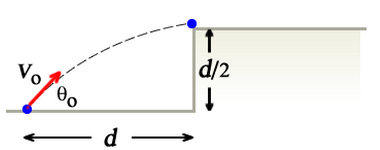
\includegraphics[scale=0.6]{Graphics/h2p3_1}
\end{center}

``(a) At what angle $\theta$ must the person throw the object and with what magnitude of the velocity $v_0$ if the object is to be exactly at the top of its flight when it reaches the ledge? Express your answer for the speed in terms of the given quantities $d$ and $g$, as needed. For the angle, enter the numerical answer in degrees.''

I first tried to solve this by starting from the kinematics equations for $x$ and $v$, but that turned out a bit painful ($d$ is unknown, $\theta$ is unknown, $t$ in unknown), so I went back and decided to use the equations we derived in lecture instead. Here they are:

\begin{align}
t_p &= \frac{v_0 \sin \alpha}{g}\\
h &= \frac{(v_0 \sin \alpha)^2}{2g}\\
t_s &= \frac{2 v_0 \sin \alpha}{g}\\
\text{OS} &= \frac{v_0^2 \sin 2\alpha}{g}
\end{align}

$t_p$ is the time to reach the apex (or p for peak); $h$ is the maximum height reached by the projectile; $t_s$ is the time until it comes back down to the $y$ coordinate it was launched from (this one is certainly not useful here), and OS is the total horizontal distance traveled.\\
The angle $\alpha$ is called $\theta$ in this problem, but they are of different names for the same thing.

Which should we use? $h$ is useful, since we know that the peak should be at $d/2$. OS is also useful, since we know that the horizontal distance should be $2d$ (not $d$! OS is the distance where it would land on the ground again, but we want it to travel exactly halfway there, to the ledge).

\begin{equation}
\frac{v_0^2 \sin^2 \theta}{2g} = \frac{d}{2}\\
\end{equation}
\begin{equation}
\frac{v_0^2 \sin 2\theta}{g} = 2d
\end{equation}

Let's try to solve these for $\theta$. Let's start with the top one:

\begin{align}
\sin^2 \theta = \frac{g d}{v_0^2}\\
\sin \theta = \sqrt{\frac{g d}{v_0^2}}\\
\theta = \arcsin \frac{\sqrt{g d}}{v_0}
\end{align}

Then there's this one:

\begin{align}
\frac{v_0^2 \sin 2\theta}{g} = 2d\\
\sin 2\theta = \frac{2 g d}{v_0^2}\\
2\theta = \arcsin \frac{2 g d}{v_0^2}\\
\theta = \frac{1}{2} \arcsin \frac{2 g d}{v_0^2}
\end{align}

These two equations both contain $d$ and $v_0$, so we should be able to solve for them:

\begin{align}
\arcsin \frac{\sqrt{g d}}{v_0} = \frac{1}{2} \arcsin \frac{2 g d}{v_0^2}
\end{align}

I'm pretty sure I've missed \emph{something} along the way, because this looks much more complex than I would have assumed this problem to be from the beginning... Either way, I solved this with computer algebra software (which is allowed, but I prefer to do everything myself to make sure that I know how to!), and found

\begin{equation}
v_0 = \sqrt{2 d g}
\end{equation}

... which is correct. We can then find the angle $\theta$,which we above stated was equal to either of the two expressions we equated above... so we stick in this value for $v_0$ and see what it turns out to equal, after simplification:

\begin{align}
&\arcsin \frac{\sqrt{g d}}{\sqrt{2 d g}}\\
&\arcsin \frac{1}{\sqrt{2}} = \ang{45}
\end{align}

Wohoo, I didn't even need to use a regular calculator for that one.\\
But wait, there's more!

``Once the object reaches the ledge it slows down with a constant deceleration and comes to a stop after sliding a distance $s$.

\begin{center}
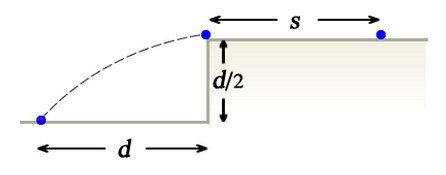
\includegraphics[scale=0.6]{Graphics/h2p3_2}
\end{center}

(b) What is the magnitude of the horizontal component of the acceleration? Express your answer in terms of the given quantities $s$, $d$, and $g$.''

The horizontal velocity is constant at $v_0 \cos \theta$ until it starts gliding. We know both $v_0$ and $\theta$, so let's call this $v_{0x}$ (we will also set $t = 0$ for simplicity):

\begin{equation}
v_{0x} = v_0 \cos \theta = \sqrt{2 d g} \cos( \ang{45}) = \frac{\sqrt{2 d g}}{\sqrt{2}} = \sqrt{d g}
\end{equation}

The rest should be easy. We use $x_0 = 0$, $v_0 = v_{0x}$ and $a_x$ as an unknown, starting at $t = 0$:

\begin{align} 
v_{0x} t + \frac{1}{2} a_x t^2 = s\\
t \sqrt{d g} + \frac{1}{2} a_x t^2 = s
\end{align}

Unfortunately, we still have a $t$ in there. We can eliminate that, since we know the initial velocity, so we can set up

\begin{align}
v_{0x} + a_x t = 0\\
t = -\frac{\sqrt{d g}}{a_x}
\end{align}

That gives us the final equation we need, after solving it for $a_x$:

\begin{align}
\left(-\frac{\sqrt{d g}}{a_x}\right) \sqrt{d g} + \frac{1}{2} \frac{\sqrt{d g}^2}{a_x} = s\\
\left(-\frac{d g}{a_x}\right) + \frac{1}{2} \frac{d g}{a_x} = s\\
-d g + \frac{1}{2} d g = s a_x\\
- \frac{1}{2} d g = s a_x\\
- \frac{d g}{2s} = a_x\\
|a_x| = \frac{d g}{2s}
\end{align}

Finally! I look forward to reading the staff's solution... I expect it to be about a third of mine in sheer length!

\section{Problem 4: Falling apple and arrow}

``An archer stands a horizontal distance $d = 50$ m away from a tree sees an apple hanging from the tree at $h = 8$ m above the ground. The archer chooses an arrow and prepares to shoot. The arrow is initially 1.5 m above the ground. Just as the archer shoots the arrow with a speed of 70 m/s, the apple breaks off and falls straight down. A person of height 2.0 m is standing directly underneath the apple. The arrow pierced the apple. Ignore air resistance, and use $g = \SI{9.81}{m/s^2}$ for the acceleration of gravity.

(a) What angle did the archer aim the arrow? Enter your answer in degrees.''

We really need to sketch this to make sure we don't screw something up re: the coordinate system, etc. Unfortunately, I draw on paper, and can't really show the picture here. (In theory I could photograph it, but I don't have a scanner. Besides, it's ugly!)

Let's first calculate the trajectory of the apple. I choose a coordinate system centered on the ground below the archer, such that $y = 0$ is below the arrow, which starts at $y_{0p} = \SI{1.5}{m}$ and $x_0 = 0$. Since both apple and arrow unfortunately begin with an a, I choose $p$ for projectile as the subscript for the arrow, and $a$ for the apple.

We then have, for the apple:

\begin{align}
x_{0a} &= \SI{50}{m} \text{ (constant)}\\
y_{0a} &= \SI{8}{m}\\
v_{y0a} &= 0\\
a_{ya} &= -g
\end{align}

So the only relevant kinematics equation for the apple is
\begin{equation}
y_{a}(t) = \SI{8}{m} - \frac{1}{2} g t^2\\
\end{equation}

Next, the arrow. Here, we need to do some decomposition, since it moves in both $x$ and $y$.

The arrow will fall at the exact same acceleration as the apple. Because they start falling the same instant, this means that they will always ``fall together'', despite the fact that the arrow has initial velocity upwards. What this means in practice is that because he hit the apple, and it started falling at the same time as the arrow, he \emph{must} have aimed \emph{exactly} at the apple when he fired.\\
This holds true regardless of the arrow's velocity, as long as it gets to the apple before it hits the ground.

Therefore, we can find the angle $\theta$ via basic trigonometry, instead of struggling with multiple unknowns in ugly equations!\\
We draw a triangle in our sketch, with the adjacent side being the horizontal $\SI{50}{m}$ to the apple, and the opposite side being the vertical $\SI{6.5}{m}$ to the apple \emph{from the arrow's initial position} of \SI{1.5}{m}. Using trigonometry, we see that

\begin{align}
\tan \theta &= \frac{\SI{6.5}{m}}{\SI{50}{m}}\\
\theta &= \arctan \frac{\SI{6.5}{m}}{\SI{50}{m}} \approx \ang{7.407}
\end{align}

That answers part (a), and simplifies things greatly for the next part. We can now calculate the arrow's trajectory without any unknowns.

\begin{align}
x_{0p} &= 0\\
y_{0p} &= \SI{1.5}{m}\\
v_{0p} &= \SI{70}{m/s}\\
v_{0px} &= (\SI{70}{m/s}) \cos \theta \approx \SI{69.416}{m/s}\\
v_{0py} &= (\SI{70}{m/s}) \sin \theta \approx \SI{9.024}{m/s}\\
a_{yp} &= -g
\end{align}

We don't really care at which velocity it hits the apple, so we have two relevant equations:

\begin{align}
x_p(t) = v_{0px} t = (\SI{69.416}{m/s}) t\\
y_p(t) = \SI{1.5}{m} + (\SI{9.024}{m/s}) t - \frac{1}{2} g t^2
\end{align}

The arrow hits the apple when their y location is equal, and $x = \SI{50}{m}$ (the apple falls straight down, with $x$ always being 50 m).

We can find $t$ from the $x$ equation for the arrow:

\begin{align}
\SI{50}{m} = (\SI{69.416}{m/s}) t\\
t = \frac{\SI{50}{m}}{\SI{69.416}{m/s}} \approx \SI{0.7203}{s}
\end{align}

Since this is the only time where the arrow is at $x = \SI{50}{m}$, it must be where it hit the apple.

``(b) How high above the person's head did the arrow hit the apple?''

We can find the $y$ coordinate easily, since we wrote a kinematic equation for that:

\begin{align}
y_a(t) = \SI{8}{m} - \frac{1}{2} g t^2 = \SI{8}{m} - \SI{2.544}{m} = \SI{5.466}{m}
\end{align}

The answer is then that minus two meters, since the question want the distance between the person's head and the apple.

\section{Problem 5: Catch}

\begin{center}
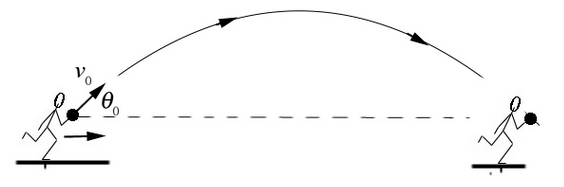
\includegraphics[scale=0.6]{Graphics/h2p5}
\end{center}

``A person initially at rest throws a ball upward at an angle $\theta_0 = \ang{70}$ with an initial speed $v_0 = \SI{15}{m/s}$. He tries to catch up to the ball by accelerating with a constant acceleration a for a time interval of 1.01 s and then continues to run at a constant speed for the rest of the trip. He catches the ball at exactly the same height he threw it. Let $g = \SI{9.81}{m/s^2}$ be the gravitational constant. What was the person's acceleration $a$ (in $\text{ m/s}^2$)?''

OK, since we know the initial velocity and angle right off the bat, let's calculate the ball's initial velocity components:

\begin{align}
v_{0x} &= (\SI{15}{m/s}) \cos(\ang{70}) \approx \SI{5.13}{m/s}\\
v_{0y} &= (\SI{15}{m/s}) \sin(\ang{70}) \approx \SI{14.095}{m/s}
\end{align}

We define $x_0 = 0$ to be the x position where he starts out, and $y_0$ to be the height the ball is as he throws it. The ball's trajectory is described by

\begin{align}
x(t) &= (\SI{5.13}{m/s}) t\\
y(t) &= (\SI{14.095}{m/s}) t - \frac{1}{2} g t^2
\end{align}

He catches the ball as $y(t) = 0$ again, so let's solve for that time:

\begin{align}
(\SI{14.095}{m/s}) t - \frac{\SI{9.8}{m/s^2}}{2} t^2 = 0
\end{align}

Using the quadratic formula $t = \frac{-b \pm \sqrt{b^2 - 4ac}}{2a}$ with $a = - \frac{\SI{9.8}{m/s^2}}{2}$, $b = \SI{14.095}{m/s}$ and $c = 0$ yields

\begin{align}
t &= \frac{-\SI{14.095}{m/s} \pm \sqrt{(\SI{14.095}{m/s})^2 - 0}}{-\SI{9.8}{m/s^2}}\\
  &= -\frac{\SI{14.095}{m/s} \pm \SI{14.095}{m/s}}{\SI{-9.8}{m/s^2}}\\
  &= \SI{2.87607}{s}
\end{align}

(ignoring the other solution, which is clearly zero, as it should be).

Thus he runs at constant speed for $\SI{2.87607}{s} - \SI{1.01}{s} = \SI{1.866}{s}$.

$t = 0$ to $t = \SI{1.01}{s}$: constant acceleration at unknown acceleration $a$.\\
$t = \SI{1.01}{s}$ to $t = \SI{2.87607}{s}$: constant speed (also unknown).\\
$t = \SI{2.87607}{s}$: catches the ball.

Using the $x(t)$ equation for the ball, he catches it after having moved \SI{14.75}{m}, which is then also the total distance he must move in the time periods above.

This causes a bit of a problem: we don't know his position when he changes to constant velocity, nor do we know the velocity. We still have enough information, though:

\begin{align}
a \cdot (\SI{1.01}{s}) &= \text{the constant velocity, after having accelerated}\\
(a \cdot \SI{1.01}{s}) \cdot \SI{1.866}{s} &= \text{distance covered at constant speed}\\
\frac{1}{2} a (\SI{1.01}{s})^2 &= \text{distance covered while accelerating}
\end{align}

We add the distances covered with the total distance covered, and solve for $a$:

\begin{align}
(\frac{1}{2} a (\SI{1.01}{s})^2) + (a \cdot \SI{1.01}{s}) \cdot \SI{1.866}{s} = \SI{14.75}{m}\\
(\frac{1}{2} a (\SI{1.02}{s^2}) + (a \cdot \SI{1.88}{s^2}) = \SI{14.75}{m}\\
a (\SI{0.51}{s^2} + \SI{1.88}{s^2}) = \SI{14.75}{m}\\
a \approx \SI{6.17}{m/s^2}
\end{align}

\section{Problem 6: Jumping off a cliff}

\begin{center}
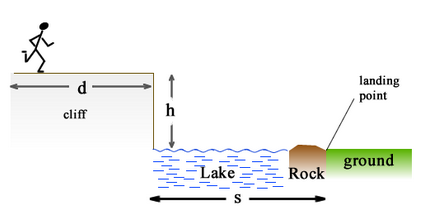
\includegraphics[scale=0.75]{Graphics/h2p6}
\end{center}

``A person, standing on a vertical cliff a height $h$ above a lake, wants to jump into the lake but notices a rock just at the surface level with its furthest edge a distance $s$ from the bottom of the cliff. The person realizes that with a running start it will be possible to just clear the rock, so the person steps back from the edge a distance $d$ and starting from rest, runs at a constant acceleration $a$ and then leaves the cliff horizontally. The person just clears the rock. Find $s$ in terms of the given quantities $d$, $a$, $h$, and the gravitational acceleration $g$. You may neglect all air resistance.''

Well, there is a typo in the problem. The person doesn't want to ``jump into the lake'', but rather wants to jump \emph{past} the lake! Either way, this problem is similar to the previous problem: the person can only accelerate (with constant acceleration, apparently) for part of the journey, and will travel the rest at constant velocity (in $x$).

Let's first look at the second part of the motion: he needs to fall $h$ meters and move $s$ meters forward in exactly the same time; the fall is at 0 initial speed and constant acceleration $-g$, while the horizontal motion is at an unknown initial speed and no acceleration, i.e. constant velocity.\\
The fall time $t_f$ can be calculated easily. Let's say $y = 0$ is on the ground, so that he starts out at $y_0 = h$:

\begin{align}
h - \frac{1}{2} g t_f^2 = 0\\
t_f = \sqrt{\frac{2 h}{g}}
\end{align}

A familiar result. This time is then exactly the time he must spend to travel the distance $s$, which means we can calculate the (average, but it is constant, so that's good) velocity:

\begin{equation}
v_x = \frac{s}{t_f} = \frac{s \sqrt{g}}{\sqrt{2h}}
\end{equation}

He must then reach this velocity $v_x$ at constant acceleration, while running the distance $d$. Let's call the time taken $t_r$, with r for run.

\begin{equation}
\frac{1}{2}a t_r^2 = d
\end{equation}

Not only that, but he must reach the velocity $v_x$ in the same time $t_r$:
\begin{equation}
a t_r = \frac{s \sqrt{g}}{\sqrt{2h}}
\end{equation}

This is all we need -- we can now solve for $s$ using these equations.

\begin{equation}
s = a t_r \frac{\sqrt{2h}}{\sqrt{g}}
\end{equation}

$t_r$ is something I made up though, so we need to solve for it in the other equation:

\begin{equation}
t_r = \sqrt{\frac{2 d}{a}}
\end{equation}

Combining the two and simplifying:

\begin{align}
s = a \sqrt{\frac{2 d}{a}} \frac{\sqrt{2h}}{\sqrt{g}}\\
s = 2\sqrt{a d} \frac{\sqrt{h}}{\sqrt{g}}\\
s = 2 \frac{\sqrt{a d h}}{\sqrt{g}}
\end{align}

... and we have our answer.

\section{Problem 7: Earth rotation and centripetal acceleration}

``The Earth is spinning about its axis with a period of 23 hours 56 min and 4 sec (a sidereal day). The equatorial radius of the Earth is $\SI{6.38e6}{m}$. The latitude of MIT (Located in Cambridge, Massachusetts) is $\ang{42;44;}$.

Note: The latitude of a point on Earth, in this case MIT, is the angle from the Equator to that point measured along the meridian of that point. In the figure below the latitude of MIT is indicated with the angle $\lambda$. (A meridian is a half of a circle that passes through the north and south poles).

\begin{center}
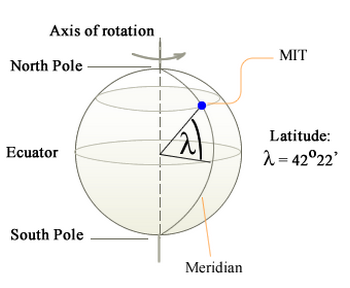
\includegraphics[scale=0.75]{Graphics/h2p7}
\end{center}

a) Find the velocity of a person at MIT as they undergo circular motion about the Earth's axis of rotation. Enter your answer in m/s.''

Let's start by converting the period $T$ to seconds, and the latitude to degrees (with decimals, instead of arcminutes):

\begin{align}
T &= 23 \cdot 3600 + 56 \cdot 60 + 4 = \SI{86164}{s}\\
\lambda &= \ang{42;22;} = \ang{42} + \frac{22}{60}^\circ = 42.3\overbar{666}^\circ
\end{align}

With the measurements in useful units, let's now calculate the ``effective radius'', so to speak. (Clearly, a person at the middle of the North Pole will have a near-zero velocity and centripetal acceleration.)

\begin{equation}
r = R_{earth} \cos(42.3\overbar{666}^\circ) \approx \SI{4.714e6}{m}
\end{equation}

The circumference at MIT's latitude is then

\begin{equation}
C = 2 \pi r \approx \SI{2.962e7}{m}
\end{equation}

So the speed is

\begin{equation}
v = \frac{C}{T} = \frac{\SI{2.962e7}{m}}{\SI{86164}{s}} \approx \SI{343.76}{m/s}
\end{equation}

``b) Find the person's centripetal acceleration. Enter your answer in $\text{ m/s}^2$.''

We can use $|a_c| = v^2/r$ very simply:

\begin{equation}
|a_c| = \frac{v^2}{r} = \frac{(\SI{343.76}{m/s})^2}{\SI{4.714e6}{m}} \approx \SI{0.0250}{m/s^2}
\end{equation}

\section{Problem 8: Relative velocity on a rotating disk}

``Particles a and b move in opposite directions with angular velocity $\omega$ around a circle of radius $L$. At $t = 0$ they are both passing through the +x axis (left figure). The angular position of particle a, $\theta$ ($>0$), is measured from the positive x-axis as shown in the right figure below. The angular position of particle b is $-\theta$.

\begin{center}
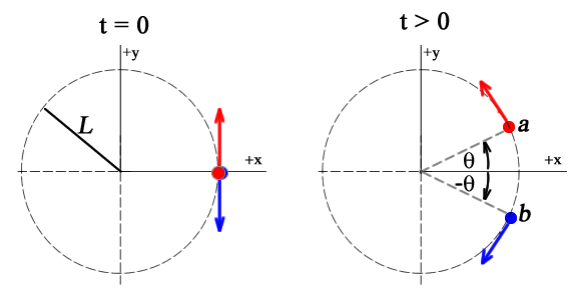
\includegraphics[scale=0.75]{Graphics/h2p8}
\end{center}

Find the x and y components of the velocity vector $\vec{v_{ab}}$, the velocity of particle $a$ relative to particle $b$. Express your answer in terms of $\omega$, $L$ and $\theta$ as needed.''

This took me a while, but once I realized how to do it, it was fairly easy.\\
The book discusses a VERY similar problem, and the exact answer is actually in the book. I didn't realize that until I had solved it, though! I had a bit of difficulty grasping a few things in their analysis, until I managed to solve it on my own.

Anyway, I'll recap my version here, even though it's similar to the book's.

First, let's define $\vec{r_a}$ and $\vec{r_b}$ as vectors from the exact center of the circle, to the respective particle they are named after. By finding the difference $\vec{r_a} - \vec{r_b}$, we find a vector pointing from $b$ to $a$, with the correct magnitude (the distance between the two). Let's call this vector $R_{ab}$:

\begin{equation}
R_{ab} = \vec{r_a} - \vec{r_b}
\end{equation}

What is this vector, in terms of components?\\
We use the unit circle definitions of the trig functions to find that. For example, for the $a$ particle, $\theta$ is positive, as is both $x$ and $y$ (at this time). Its $x$ position can be found as $L \cos \theta$, and $y$ position as $L \sin \theta$, by some basic trigonometry. (Draw it and try to calculate the components if you don't see it.)\\
The same applies to $\vec{r_b}$, except $\theta$ is negative. That makes the $y$ coordinate negative, as $\sin(-y) = -\sin(y)$, though $\cos(-x) = \cos(x)$ so nothing changes there. All in all we have

\begin{align}
\vec{r_a} = L \cos \theta \hat{x} + L \sin \theta \hat{y}\\
\vec{r_b} = L \cos \theta \hat{x} - L \sin \theta \hat{y}
\end{align}

the vector $R_{ab}$ is then found as the difference, as shown above:

\begin{align}
\vec{R_{ab}} = L \sin \theta \hat{y} - (-L \sin \theta \hat{y}) = 2 L \sin \theta \hat{y}
\end{align}

The $x$ part cancels out. If you sketch the problem (or look at the provided sketch) and imagine the particles' motion, this should be intuitive.

The only step remaining is to find the velocity vector instead of the position vector. This is simply done by taking the time derivative of the above vector.

\begin{align}
\vec{V_{ab}} = \frac{d}{dt} \vec{R_{ab}} = 2 L \frac{d\theta}{dt} \cos \theta \hat{y}
\end{align}

We get a $\displaystyle \frac{d\theta}{dt}$ outside because of the chain rule. By convention, we write that simply as $\omega$, so all in all we have:

\begin{align}
\vec{V_{ab}} &= 2 L \omega \cos \theta \hat{y}\\
{V_{ab}}_x &= 0\\
{V_{ab}}_y &= 2 L \omega \cos \theta
\end{align}

And we are done!

\end{document}